\documentclass[10pt,english]{article}
\usepackage{bookmark}
\usepackage{geometry}
\usepackage{anyfontsize}
\usepackage{lmodern}
\usepackage{lipsum}
\usepackage{sectsty}
\usepackage{amsmath}
\usepackage{amssymb}
\usepackage[T1]{fontenc}
\usepackage[utf8]{inputenc}
\usepackage[explicit]{titlesec}
\usepackage[sfdefault]{inter}
\usepackage{sfmath}
\usepackage{hyperref}
\usepackage{enumitem}
\usepackage{listings}
\usepackage[final]{graphicx}
\usepackage{subfig}
\usepackage{array}
\usepackage[table]{xcolor}
\usepackage{tikz}
\usepackage{graphicx}
\usepackage{csvsimple}
\graphicspath{{./images/}}
\usepackage[explicit]{titlesec}


\linespread{1.2}
\title{\huge{\textbf{Spotting}}}
\author{
    \\\\
    David Hermanto\\
    \small 3808127\\
    \\
    Rafat Mahiuddin\\
    \small 3897093\\
    \\
    Harry Porter\\
    \small 3888604\\
    \\
    Adrian Rebellato\\
    \small 3889401\\
    \\
    Myeonghoon Sun\\
    \small 3774430\\
    \\\\
}
\date{}

\begin{document}

\maketitle
\thispagestyle{empty}
\clearpage

\vspace*{\fill}
\begin{center}
\includegraphics[scale=0.1]{images/9DDC331C-9A71-4E19-AECC-54D8ED6C2240.png}
\end{center}
\vfill
\thispagestyle{empty}

\clearpage

\pagenumbering{arabic}

\section*{Solution}

In this section, we first discuss the components and architecture of our software, then our methodology with respect to meeting the project requirements.

% Where should this go? Probably interspersed throughout the report.
% Positions the work within the literature.
% Compares the project to other appropriate state-of-the art methods.

\subsection*{Structure}

% Technical description of project:
% Software, launch files, configuration, and implementation.
% Description of the implemented software.
%   Requires:
%   - Excellent and complete technical description of the ROS package components.

The following packages are entirely our creations, outside the Python and ROS dependecies used in their implementation.

%  spot ros and the spotters program. The movement package allows for a standradised set of methods to execute robot mvoement in a controlled, and centralised manner. The movement package also allows for robot safety, since only the spot move should move the motors on spot, spot will always stop moving if that node is killed.

\begin{itemize}[noitemsep]
    \item \texttt{spot\_compose} Entry point package used to execute Spotter's dependencies.
    \item \texttt{spot\_conductor} Conducts higher order actions in a synchronised fashion while acting as a gatekeeper to the rest of the architecture. Currently, the \texttt{Conductor} is tasked with camera calibration and orchestrating a good initialisation procudure for occupancy grid generation. It is also capable of enforcing the robot's desired behaviour throughout execution, however this functionality is not fully implemented yet.
    \item \texttt{spot\_cartographer} The \texttt{Cartographer} is responsible for managing the diverse library of maps created by our slam algorithm. As our operations must be persitent across maps, it is important to have a module that manages these changes directly. The \texttt{Cartographer} also controls the flow of point cloud data to the mapping pipeline.
    \item \texttt{spot\_geography} The geography package is a collection of pipelines responsible for filtering, evaluating, storing and processing point clouds. The primary purpose for the geography pipeline is to take in a point cloud stream and convert it to a usable occupancy grid for navigation. The geography pipeline depends on the \texttt{octomap} ROS package to create, store and load octrees based on their proposed \texttt{octreee} encoding algorithms. The usage of \texttt{octomap} as a dependency and possible replacements are discussed later on in this report.
    \item \texttt{spot\_move} represents a cohesive package for all of Spot's navigation. Every function acts as an interface between \dots The \texttt{Navigator} recevies a heavily pre processed two-dimensional occupancy grid with the objective of creating a safe path around obstacles on that grid. The primary path planner used by the \texttt{Navigator} is \texttt{D* Lite}, which allows for efficient recomputation of the path to support remapping dynamic environments.
    \item \texttt{spot\_sensor\_relay} takes adavantage of a number of iPhone sensors to enable robotic navigation. As Spotters utilises the sensor relay heavily, this allows us to decouple our alogrithms so that they may be executed over a large number of robotic platforms. When the sensor relay is booted, it creates a server and encoding pipeline to ready video frames for transport. Each pipeline runs on a separate thread, and jobs are published to a common buffer. Alongside the encoding and server pipelines, we also define custom IMU drivers for the Spotters project.
    \item \texttt{spot\_imu} listens to, parses and processes IMU data published by the sensor relay. The primary purpose of this package is to enusre the data is being published in the ROS standard.
    \item \texttt{spot\_navigator} is responsible for analysing a preprocesed occupancy grid, determining the robot's localisation status, planning appropriate behaviour given this status and other information, and planning the shortest path to a given goal node, taking into account all known obstacles. Given that the environment may change constantly as new features are identified and the \texttt{octree} point cloud updated, the navigator must implement an effiecent way of computing the shortest path. To do this, a \texttt{D* Lite} algorithm is used, which allows us to only recompute the portion of the map that has changed. The navigator also performs a lazy evaluation of the environment, which allows it to only replan paths in the robot's immediate vicinity, rather then recomputing the entire path for every map update.
\end{itemize}

We also modified some third party packages for use in this project. These are listed below.

\begin{itemize}[noitemsep]
    \item \texttt{spot\_slam} contains a ROS-based implementation of \texttt{ORB-SLAM3}. Source modifications allowed us to extend the publishing capabilities of the package to include system state and localisation data. This is then used by a wide variety of packages to determine whether Spot is currently healhty, or has lost it local environment. In addition,
    \item \texttt{spot\_ros} contains a collection of packages that allows for a standard interface with the Spot programming environment. A number of these packages have been modified to work alongside the Spotters project.
    \item \texttt{spot\_description} containts extended URDF files provded by Boston Dynamics to be compatible with our systems. This included adding origin and camera links and joints to make the body move as SLAM localises the camera frame of reference. Spot's visual mesh was also extended by including a three-dimensional model of an iPhone on top of his forehead, which was exported using Blender.xten
    \item \texttt{spot\_viz} Modifications included the addition of our own rviz configuration files.
\end{itemize}

The following packages are sourced entirely from a third party, where we have made no modifications as part of our project.

\begin{itemize}[noitemsep]
    \item \texttt{spot\_wrapper} is a wrapper around the Spot SDK. It allows for safe programmatic access to the BosDyn SDK through a standardised set of protocols. Handles lease and motor safety and additional setup configurations.
    \item \texttt{spot\_msgs} defines custom messages for a variety of ROS services, action servers and messages to control spot using ros.
    \item \texttt{spot\_cam} is a dedicated package used to handle the Spot camera extension. We do not use this at present.
    \item \texttt{spot\_driver} lies above the wrapper to manage the Spot ROS runtime. A key functionality involves delegating and piping incoming commands to the approapiate wrapper methods while ensuring errors are handled appropriately.
    \item \texttt{octomap\_server} provides the \texttt{octree} implementation for our program. Octomap exposes methods to save and load the map via their own encoding standard, which is designed to store large point cloud maps. The usage of octomap and its suitability will be disucussed later on in the reprot.
    \item \texttt{usb\_cam} allows us to load a Linux video device to a ROS image stream.
\end{itemize}

\clearpage

\subsection*{Architecture}

% Description of the of Robot Software Architecture.
% Excellent and complete.

% Justification of the choice of Robot Software Architecture.
%   Requires:
%   - Excellent justification of the Robot Software Architecture.
%   - Well-supported reasoning.



\vspace*{\fill}
\begin{center}
    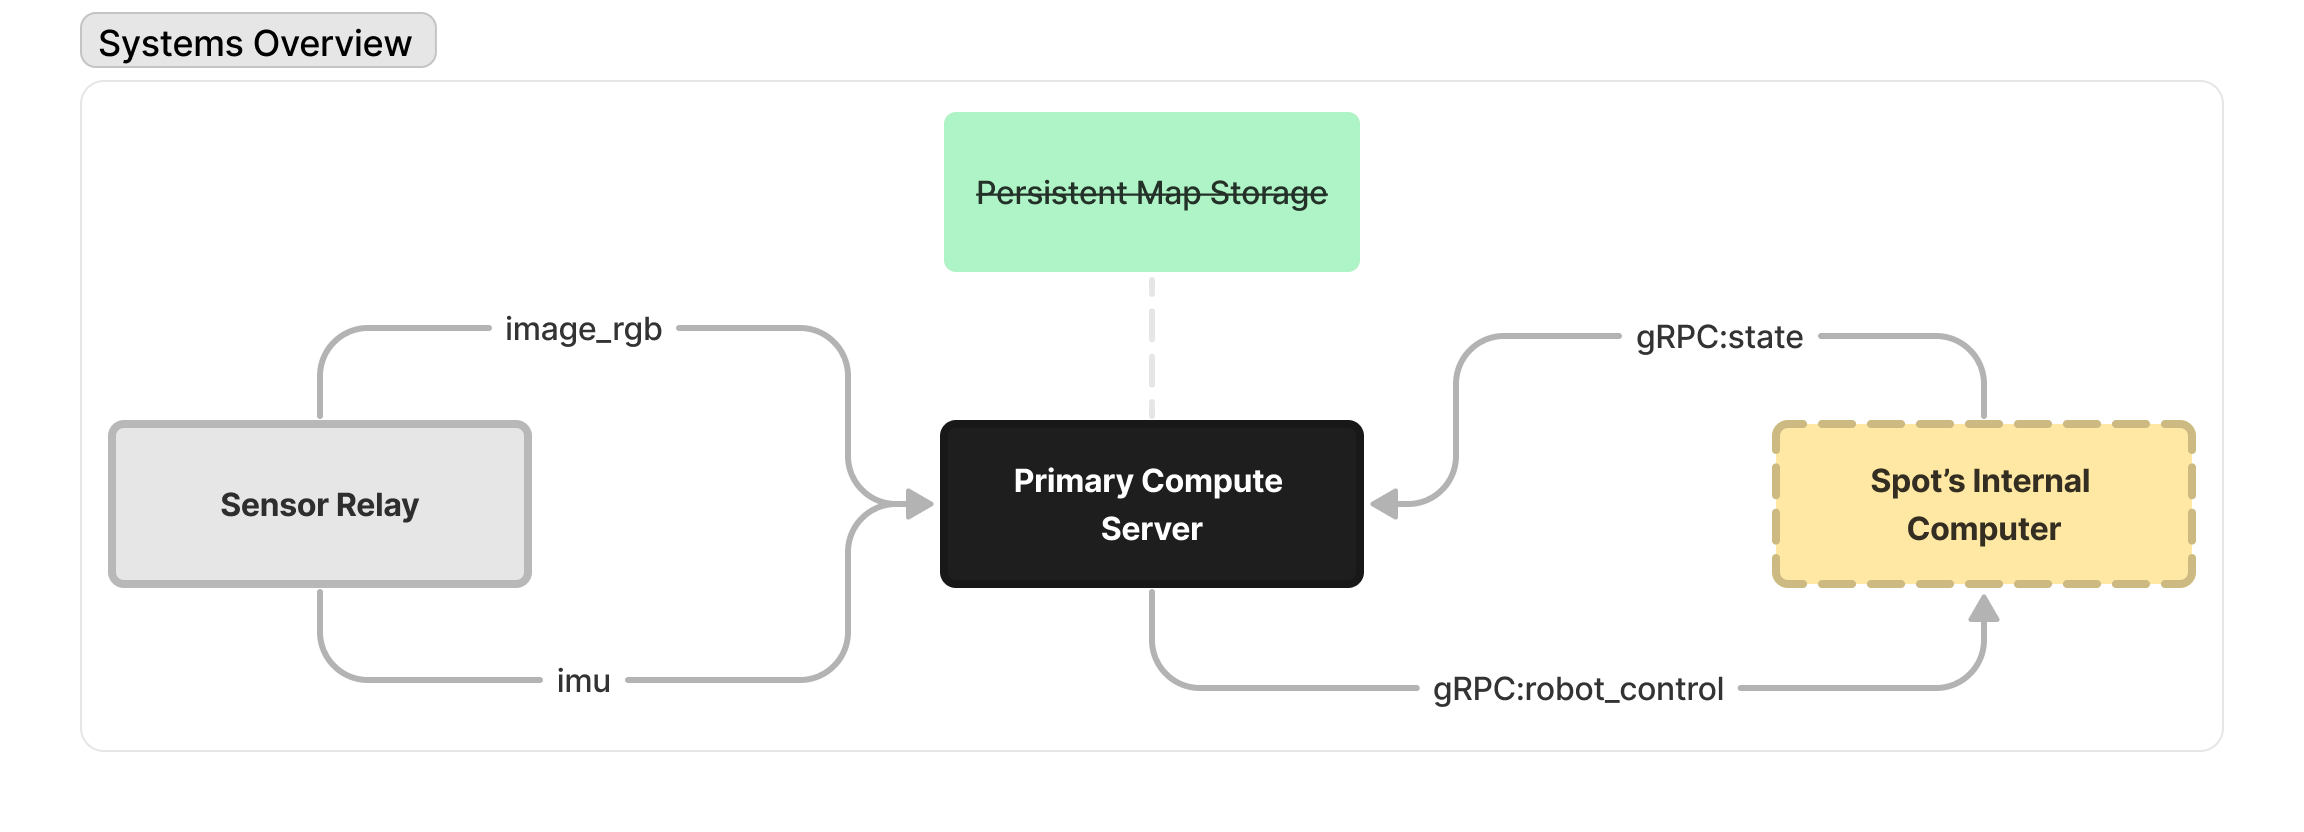
\includegraphics[width=\textwidth]{images/Systems Overview.png}
\end{center}

\begin{center}
    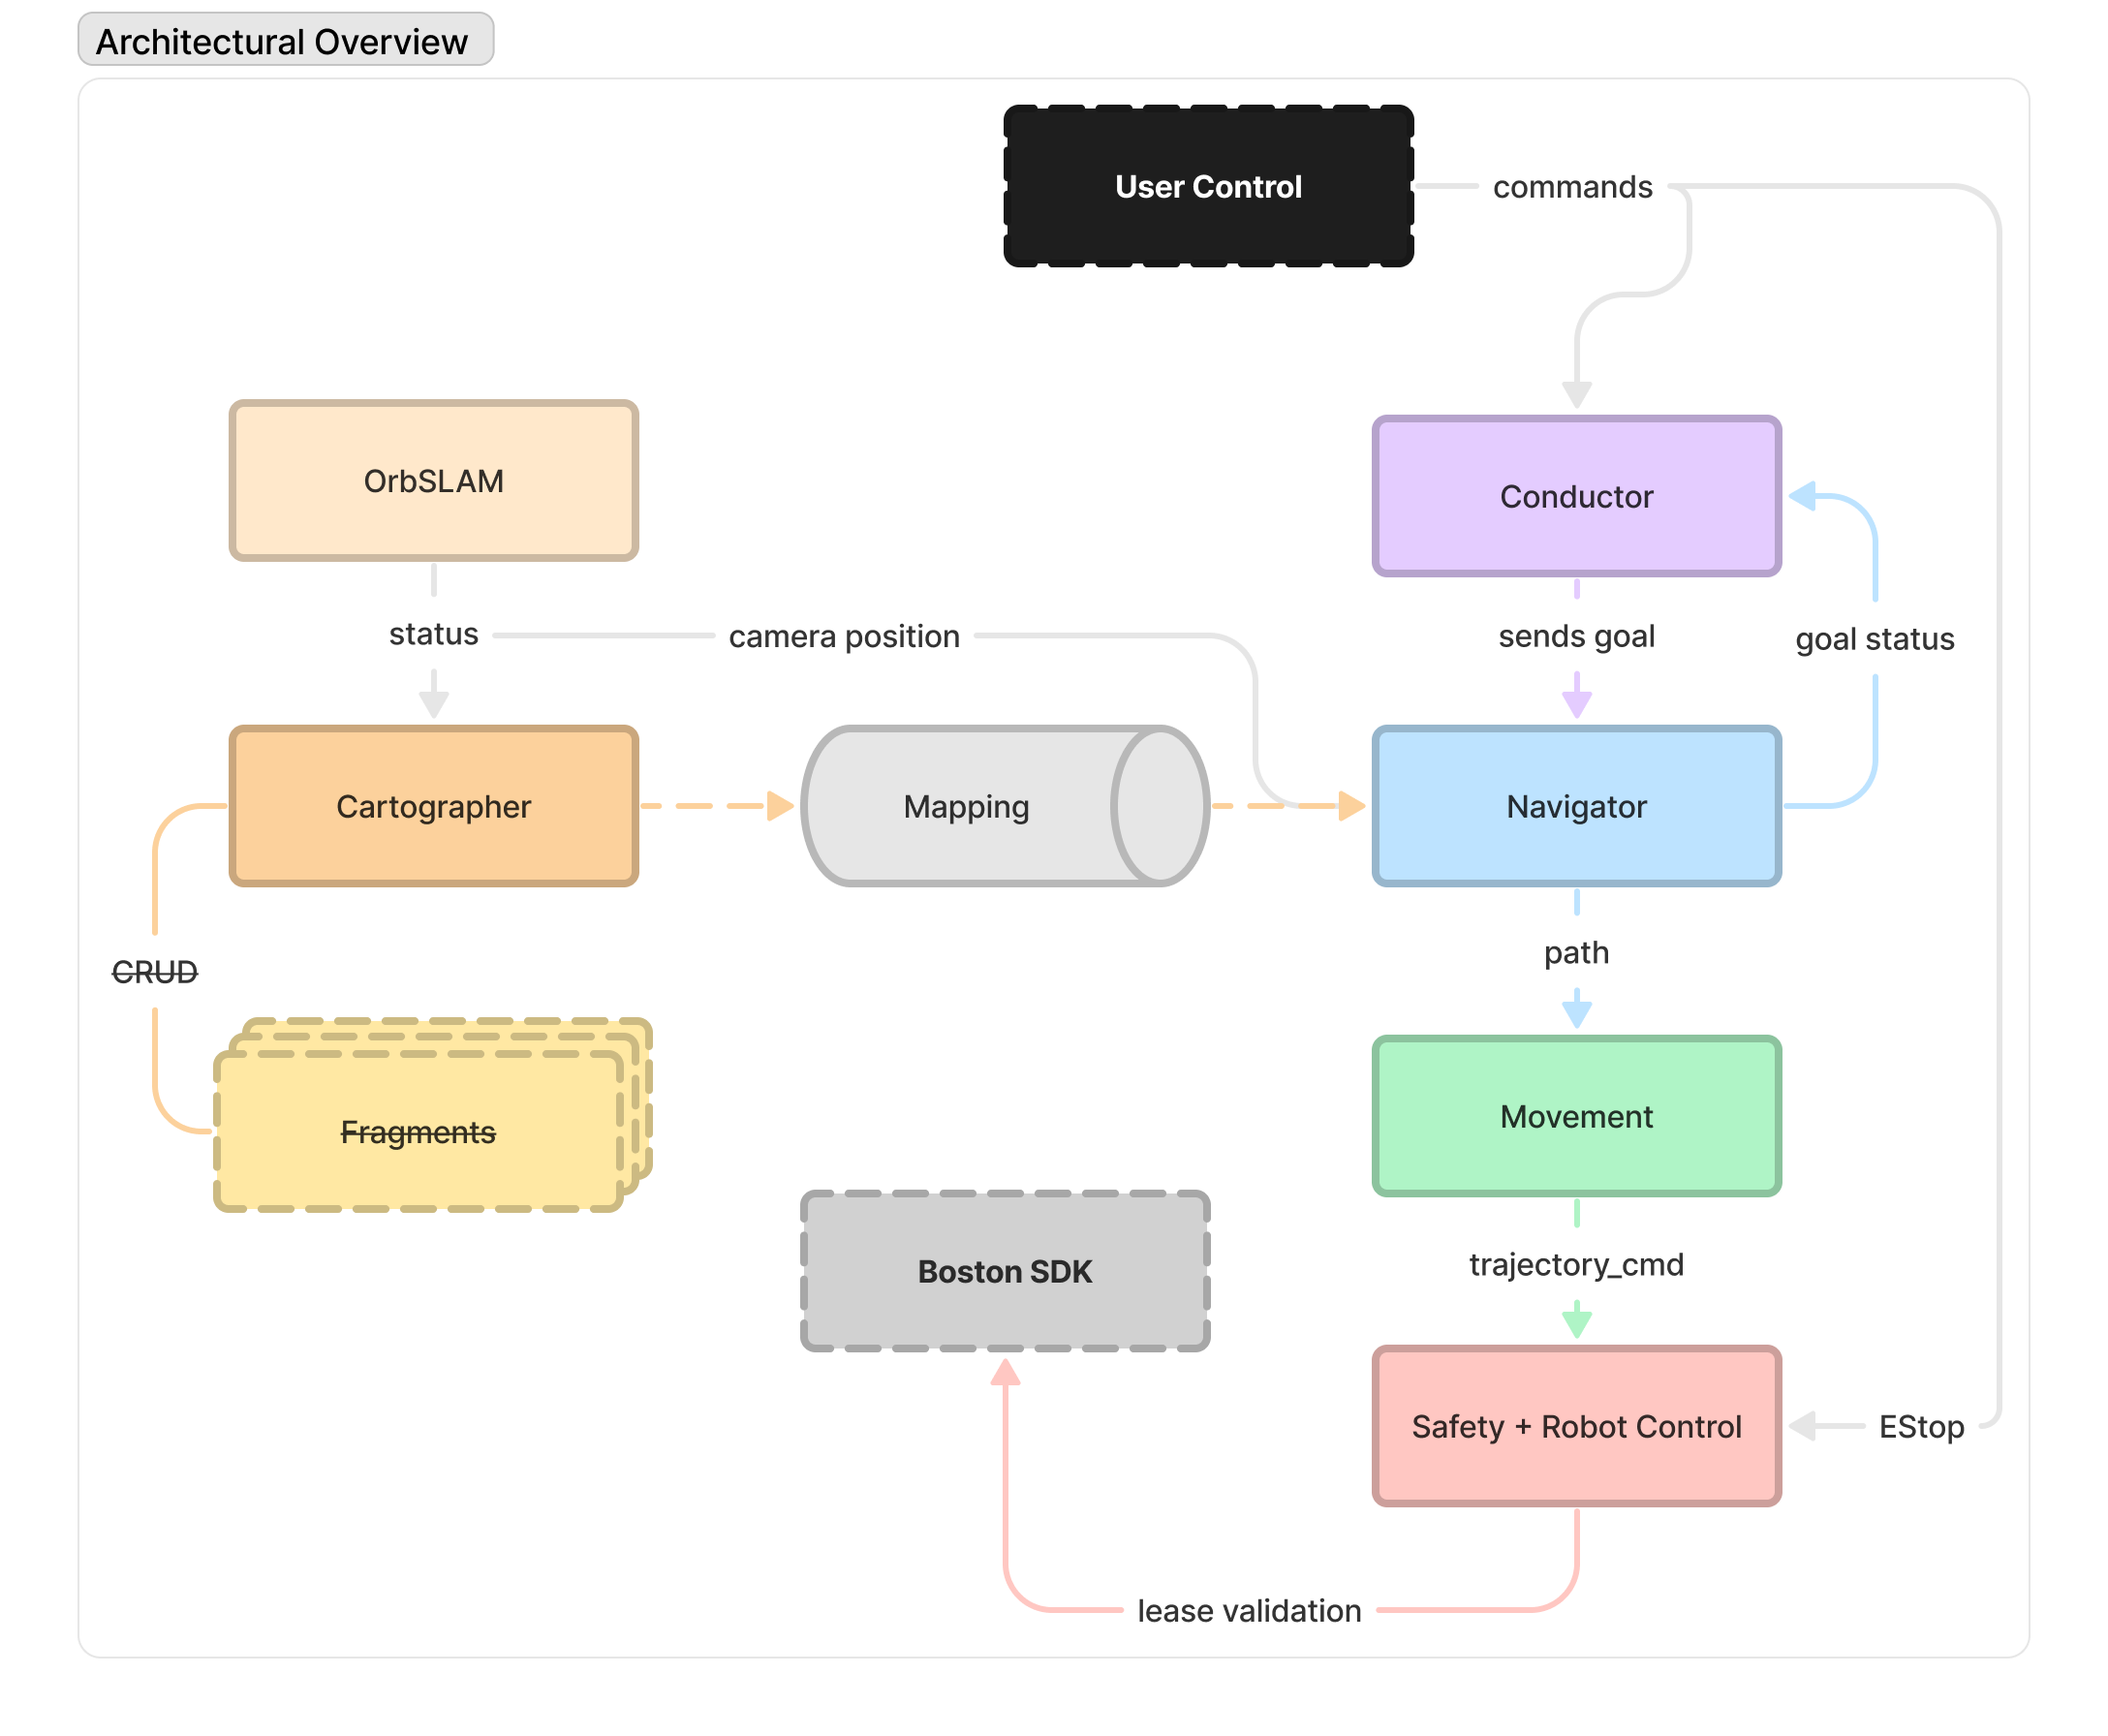
\includegraphics[width=\textwidth]{images/Architectural Overview.png}
\end{center}

\clearpage

Spotters follow a three layered architecture to establish a clear hierarchy of control within the system. The conductor is the highest level process in our system and can be associated with the deliberative layer. The conductor makes decisions based on the robot's current state and the condition of the world. An example of this may be the conductor’s ability to realize when Spot is on a portion of the unknown map. In which case, it will make the higher order decision to relocalise or build a higher resolution map using recovery behaviors. Other examples include when the robot just booted up and a map needs to be initialized before being able to navigate.

The executive (or sequencing) layer describes the second layer of our 3 layer architecture. Modules within this layer include the cartographer, navigator and the geography pipeline. Accordingly, modules within this layer are responsible for coordinating the reactive behaviors into a more complex sequence of actions. For example, the navigator must actively respond to
drastic changes in the map. These changes can include the entire map being reset, merged or scaled at different portions. Additionally, the geography pipeline will actively mutate the map based on changes in the robot's location and its corresponding environment. The navigator is tasked with planning in this dynamic environment, and does so through reactive Pose messages. These poses are chained together to create a valid navigable path the robot moves towards. Pose messages are then executed by lower level modules such as Spot Move.

Similarly, The cartographer follows the reactive standard characterized by the executive layer. More specifically, the cartographer listens for changes in localisation status and unusual additions and subtractions to the tracked point cloud and decides how the point cloud should be stored. For example, the cartographer will attempt to clear the octree if there are any significant changes in the SLAM system. However, the cartographer is yet to be fully implemented, and the full implementation of the cartographer will include storing the entire instances of the octree into `fragments'. As the ORB-SLAM algorithm switches between maps, fragments will be merged, deleted and created to correspond to this change. These fragments can then be stored in memory mapped files for quick state persistence when the robot boots up.

The lowest layer of our architecture can be classified into the reactive layer. Modules in this layer may include Spot Move and Spot's internal computer. Although there are even lower levels, from the context of our program, these modules control the motion of the robot directly. Accordingly, Spot Move responds to external messages through pre-determined behaviors and Spot's internal computers perform object avoidance based on incoming sensor data.

% \vspace*{\fill}
\begin{center}
    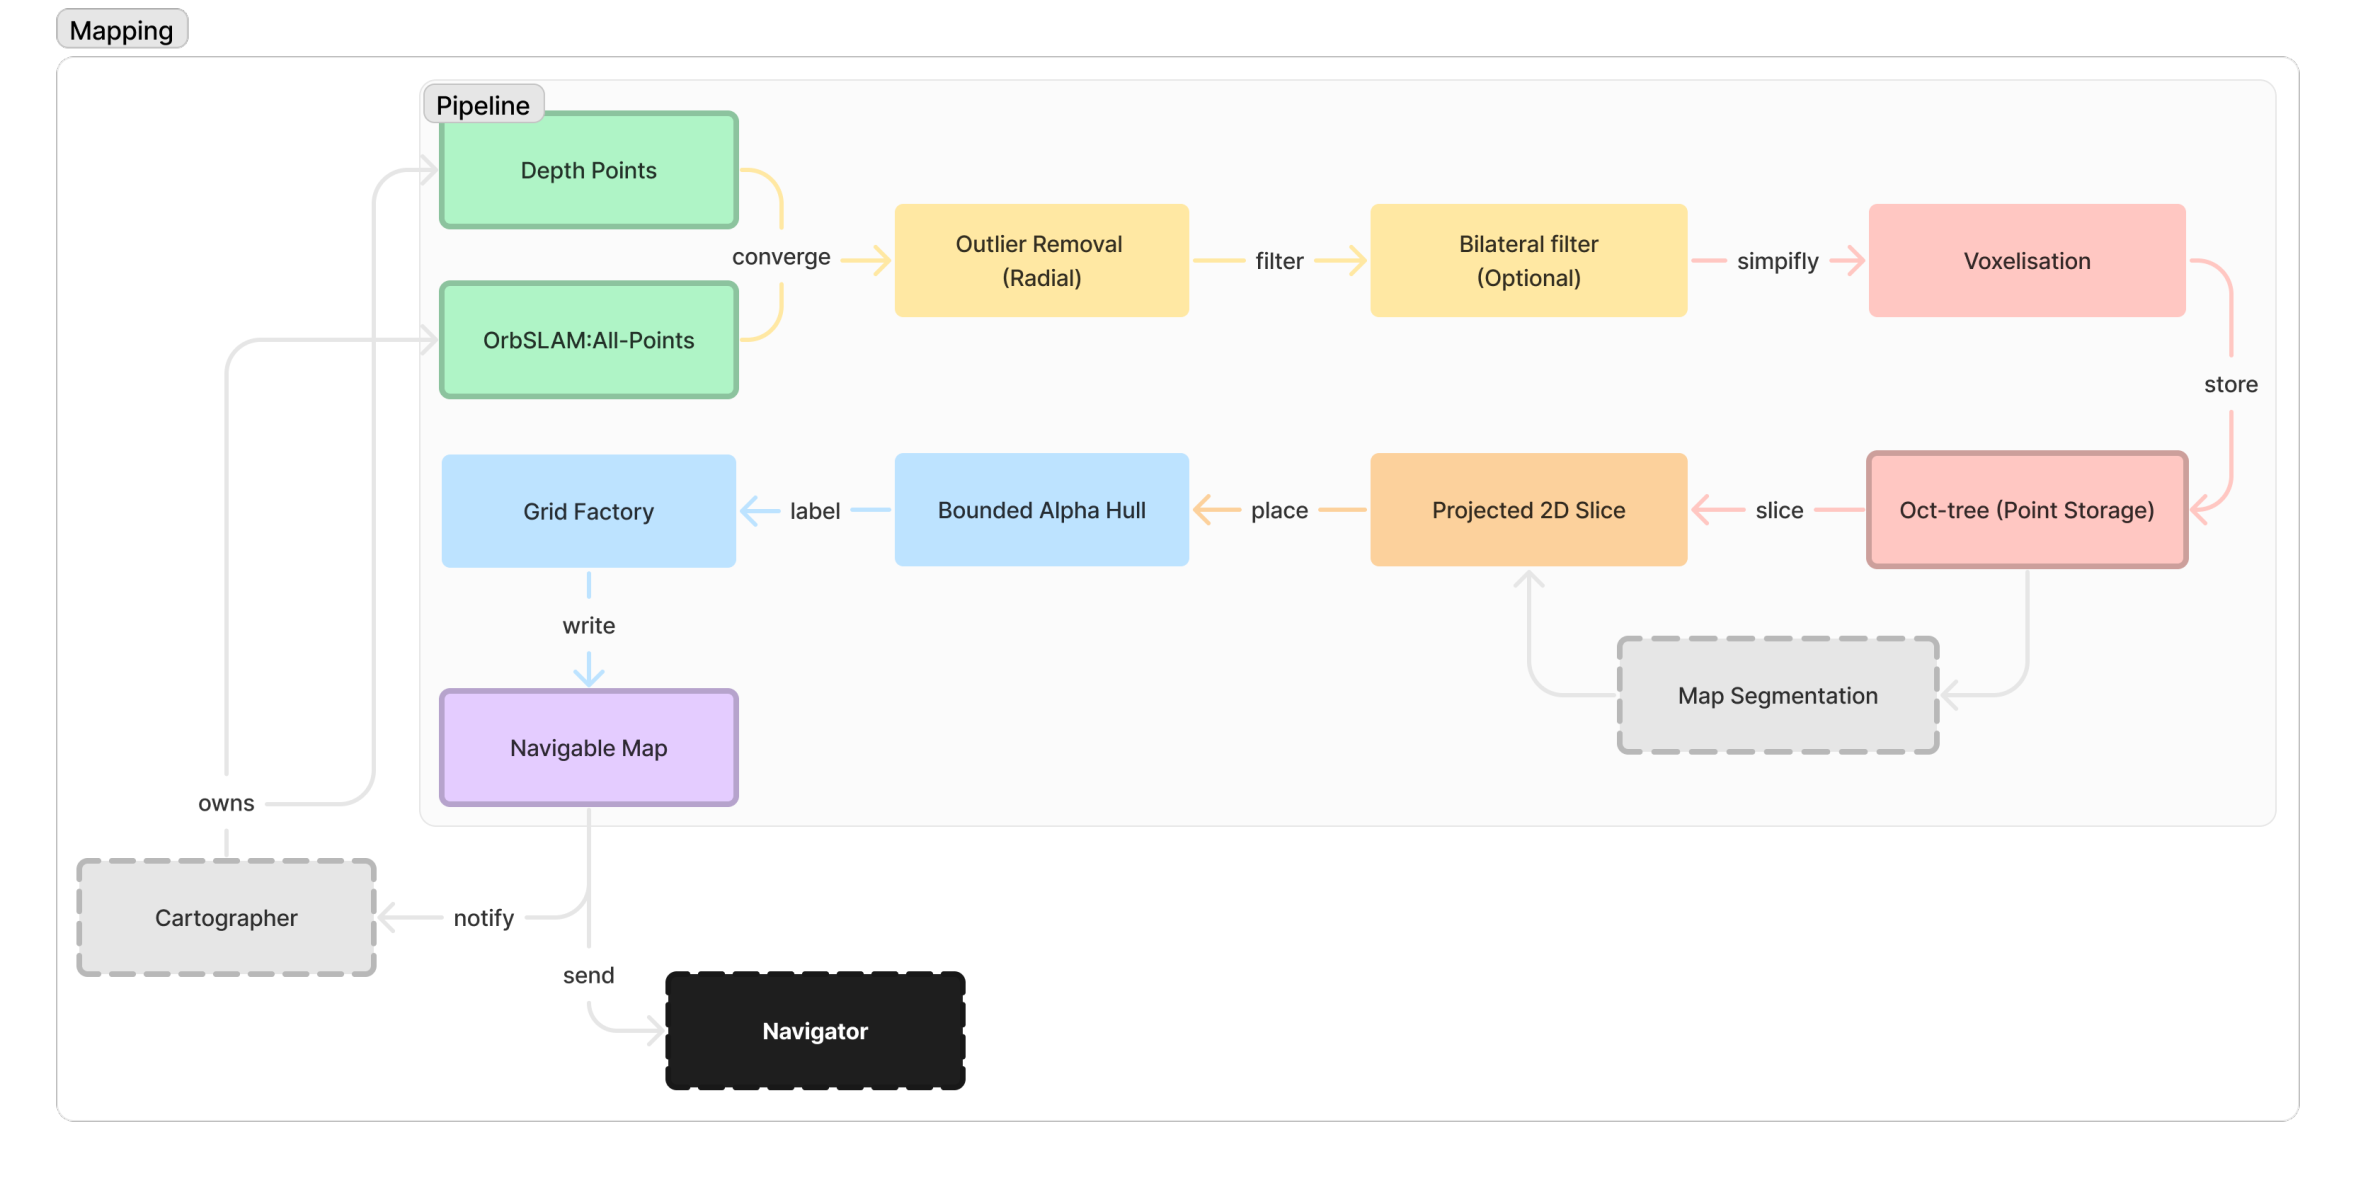
\includegraphics[width=\textwidth]{images/Mapping.png}
\end{center}

\begin{center}
    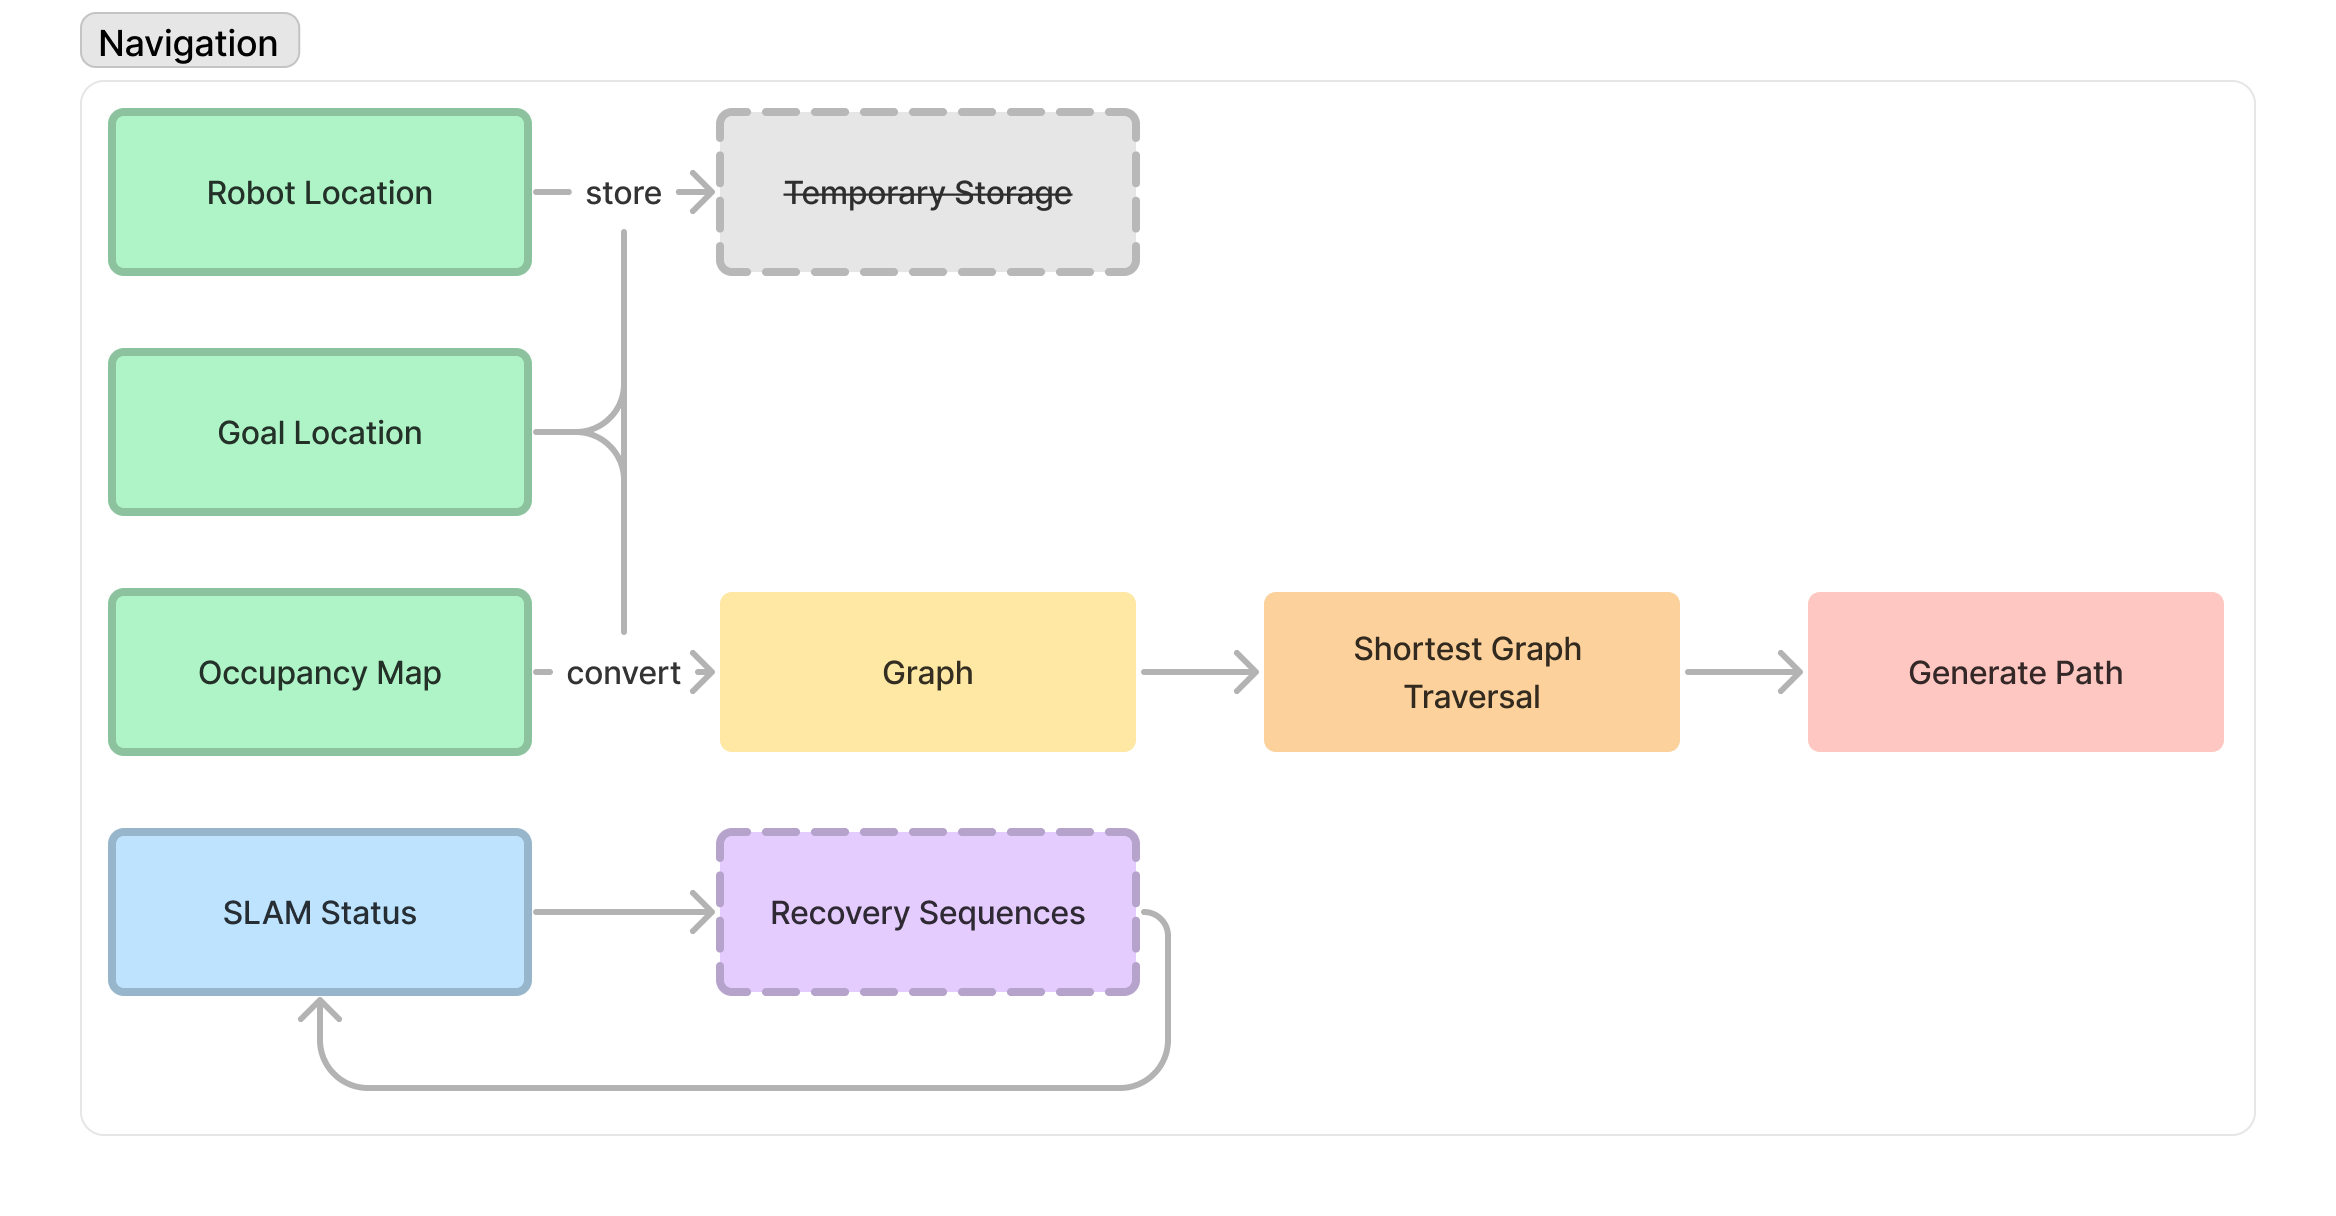
\includegraphics[width=\textwidth]{images/Navigation.png}
\end{center}

\begin{center}
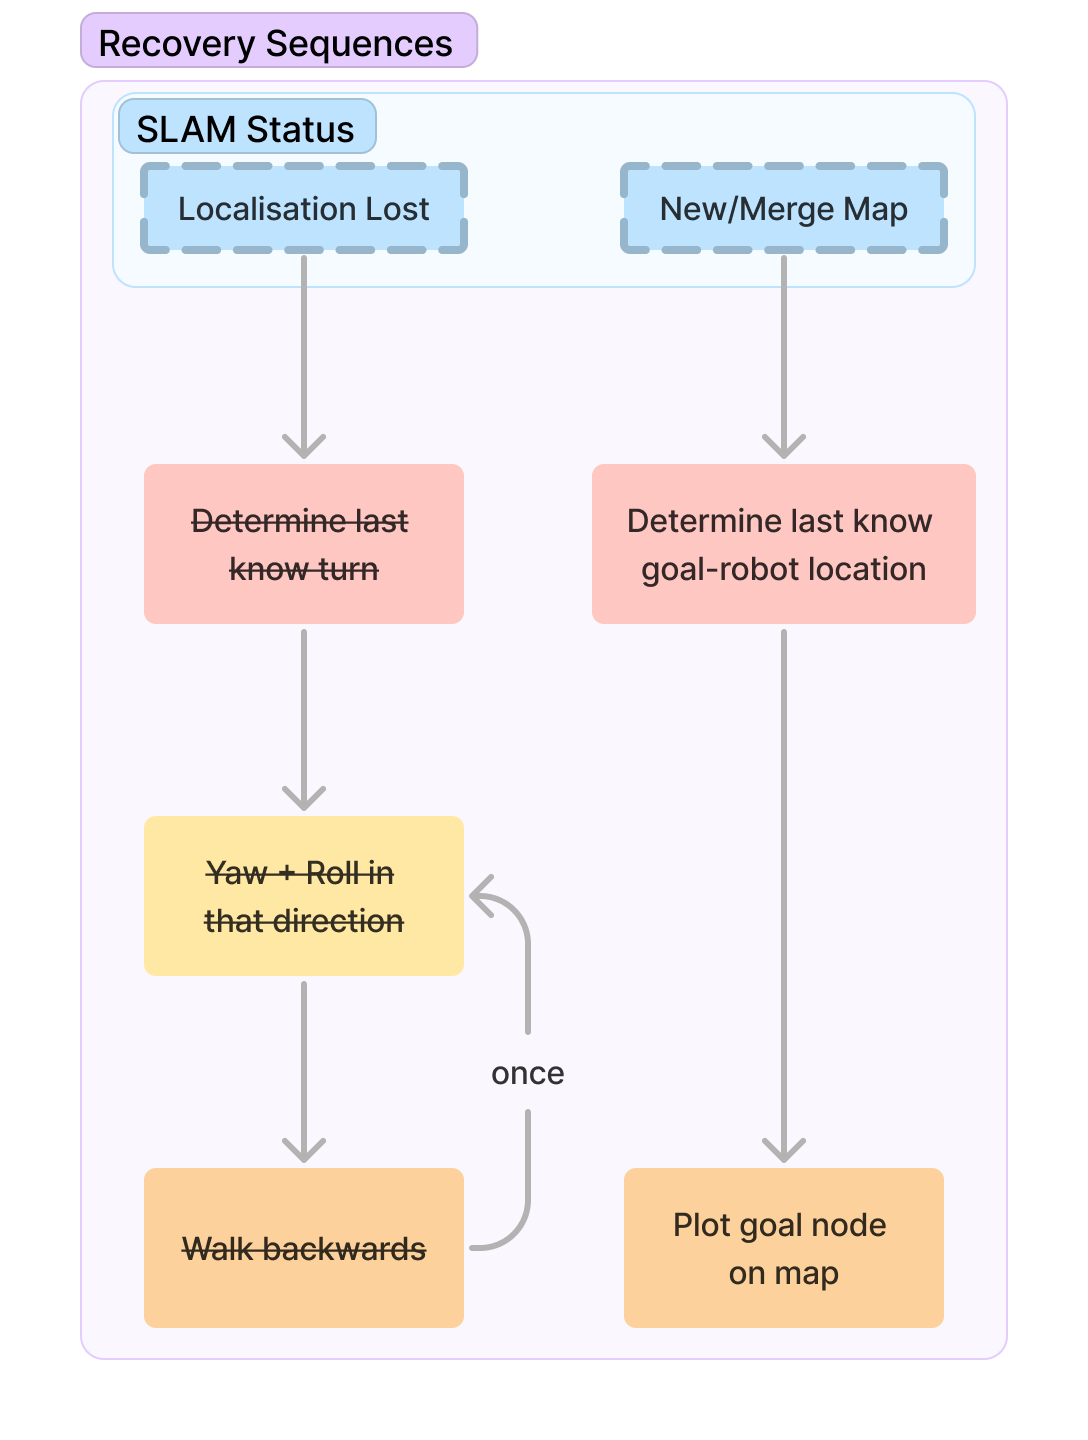
\includegraphics[width=\textwidth]{images/Recovery Sequences.png}
\end{center}


\clearpage

\subsection*{Methodology}

% Describe methodology and approach towards completing the negotiated requirements of the project.
%   Requires:
%   - Excellent description of methodology.
%   - Provides a complete picture of how the project is completed.

Here we discuss the intended and implemented behaviours of all our custom packages, and how they fit into the overall pipeline to produce navigation over an occupancy grid derived from visual information.

\subsubsection*{Localisation \& Mapping}

Our localisation and mapping processes are based on the \texttt{ORB-SLAM3} algorithm [1], with the utilization of the Open3d library and Octomap package. % Need to reference the repository.
Orb Slam3 detects features in images, and tracks them as a point cloud. The initial projection of these features in unreliable, but as the same features are tracked between moving frames, the projection accuracy increases. From the SLAM algorithm we get decent localisation, and a 'sparse' point cloud containing the SLAM features. We have made significant progress integrating both IMU data, as well as SPOT's depth cloud data into the SLAM algorithm, but at the time of this report, it is operating using only a smart-phone monocular camera.

The camera we used runs at 30 frames per second. Under normal operation this means our algorithm recieves point cloud data 30 times a second. This data can be integrated into the pre-existing point cloud map, usually resulting in improved accuracy, or cause the creation of a new one when it contains too many unrecognised points. At a slower pace, roughly once a second, the receipt of a point cloud triggers the mapping of all pre-existing point-cloud points. This cloud is filtered for significance via neighbour checking, and voxelized in an Octtree data structure provided by Octomap. The ground plane of this octree is then detected. This ground plane is a `best fit' planar surface that can be up-to 15 degrees off vertical, and it will remove a configured height of point cloud data from the base of the octree.

Spot has it's own odometry pipeline, which could potentially conflict with the localization data provided by SLAM. Rather than superceding SPOT's own propriatary odometry, we decided to model our own localization system by moving our map relative to spot (rather than moving spot relative to our map). SLAM's localization provides us with the position of the camera inside a point-cloud. Our Point cloud 'origin', and our map, are then added to SPOT's TF tree as a child of the camera, rather than parent of SPOT. A localization update calculated by SLAM, then moves the point cloud, relative to the camera. As an example, if the slam algorithm localization determines that the camera is at (50, 100), the 'origin' frame will be translated to (-50, -100) relative to it's parent, the camera. The end effect is our point cloud, map, and occupancy grid moving in tandem with SPOT, without it ever conflicting with SPOT's odometry. Translations from this frame to SPOT's body can still be performed by traversing the TF tree regularly. In other words, our map moves under SPOT, rather than SPOT moving over our map.

\vspace*{\fill}
\begin{center}
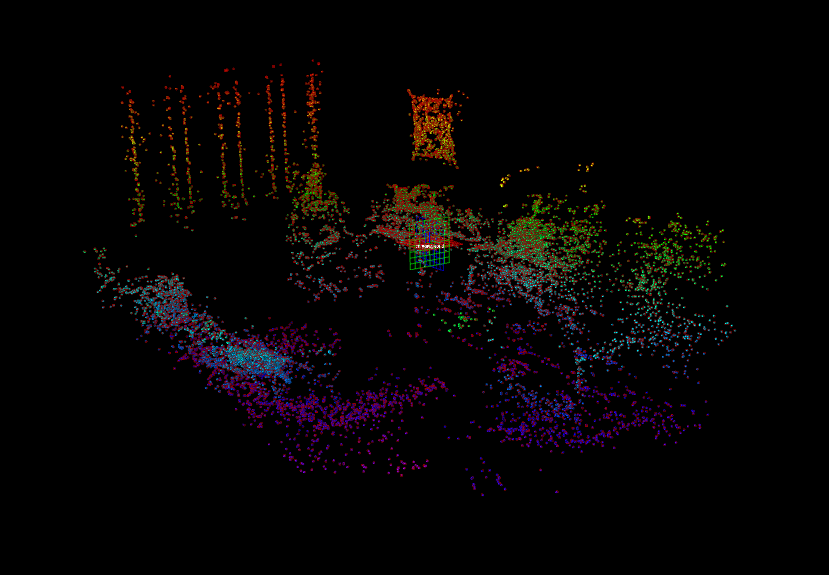
\includegraphics[width=0.5\textwidth]{images/RafCloud.png}
\linebreak
\linebreak
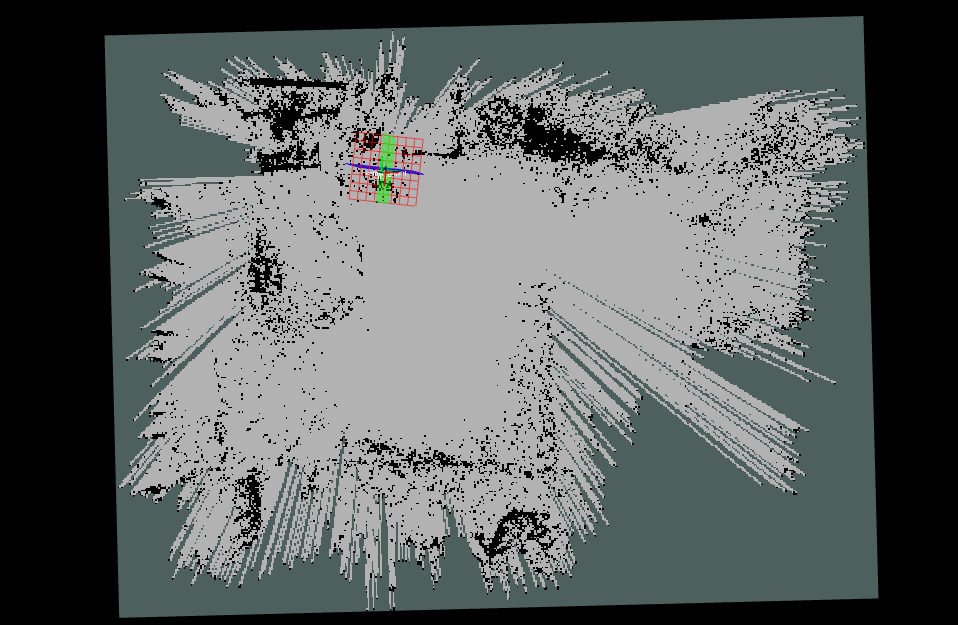
\includegraphics[width=0.5\textwidth]{images/RafGridNoFilter.png}
\linebreak
\linebreak
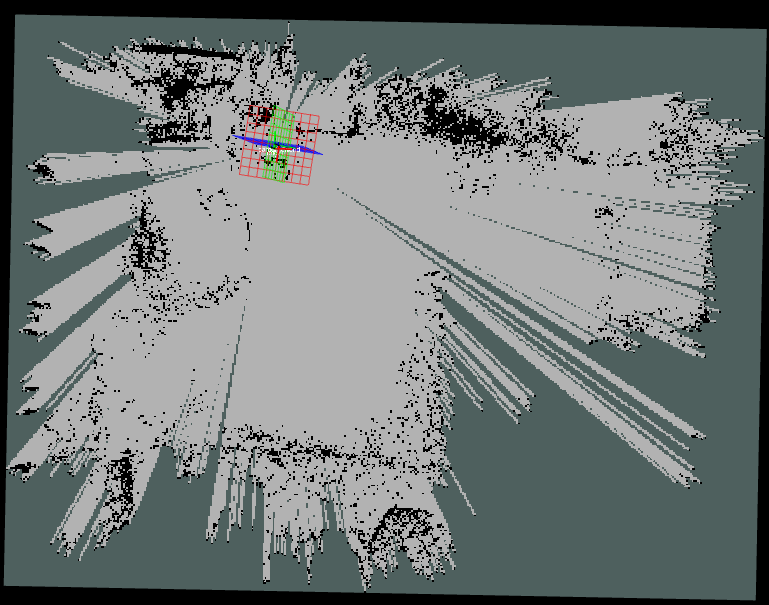
\includegraphics[width=0.5\textwidth]{images/RafGridAggressiveFilter.png}
\linebreak
\linebreak
\text{\texttt{ORB-SLAM3} point cloud; two-dimensional slice before and after filtering.}
\end{center}
\vfill
\thispagestyle{empty}

\clearpage

\vspace*{\fill}
\begin{center}
    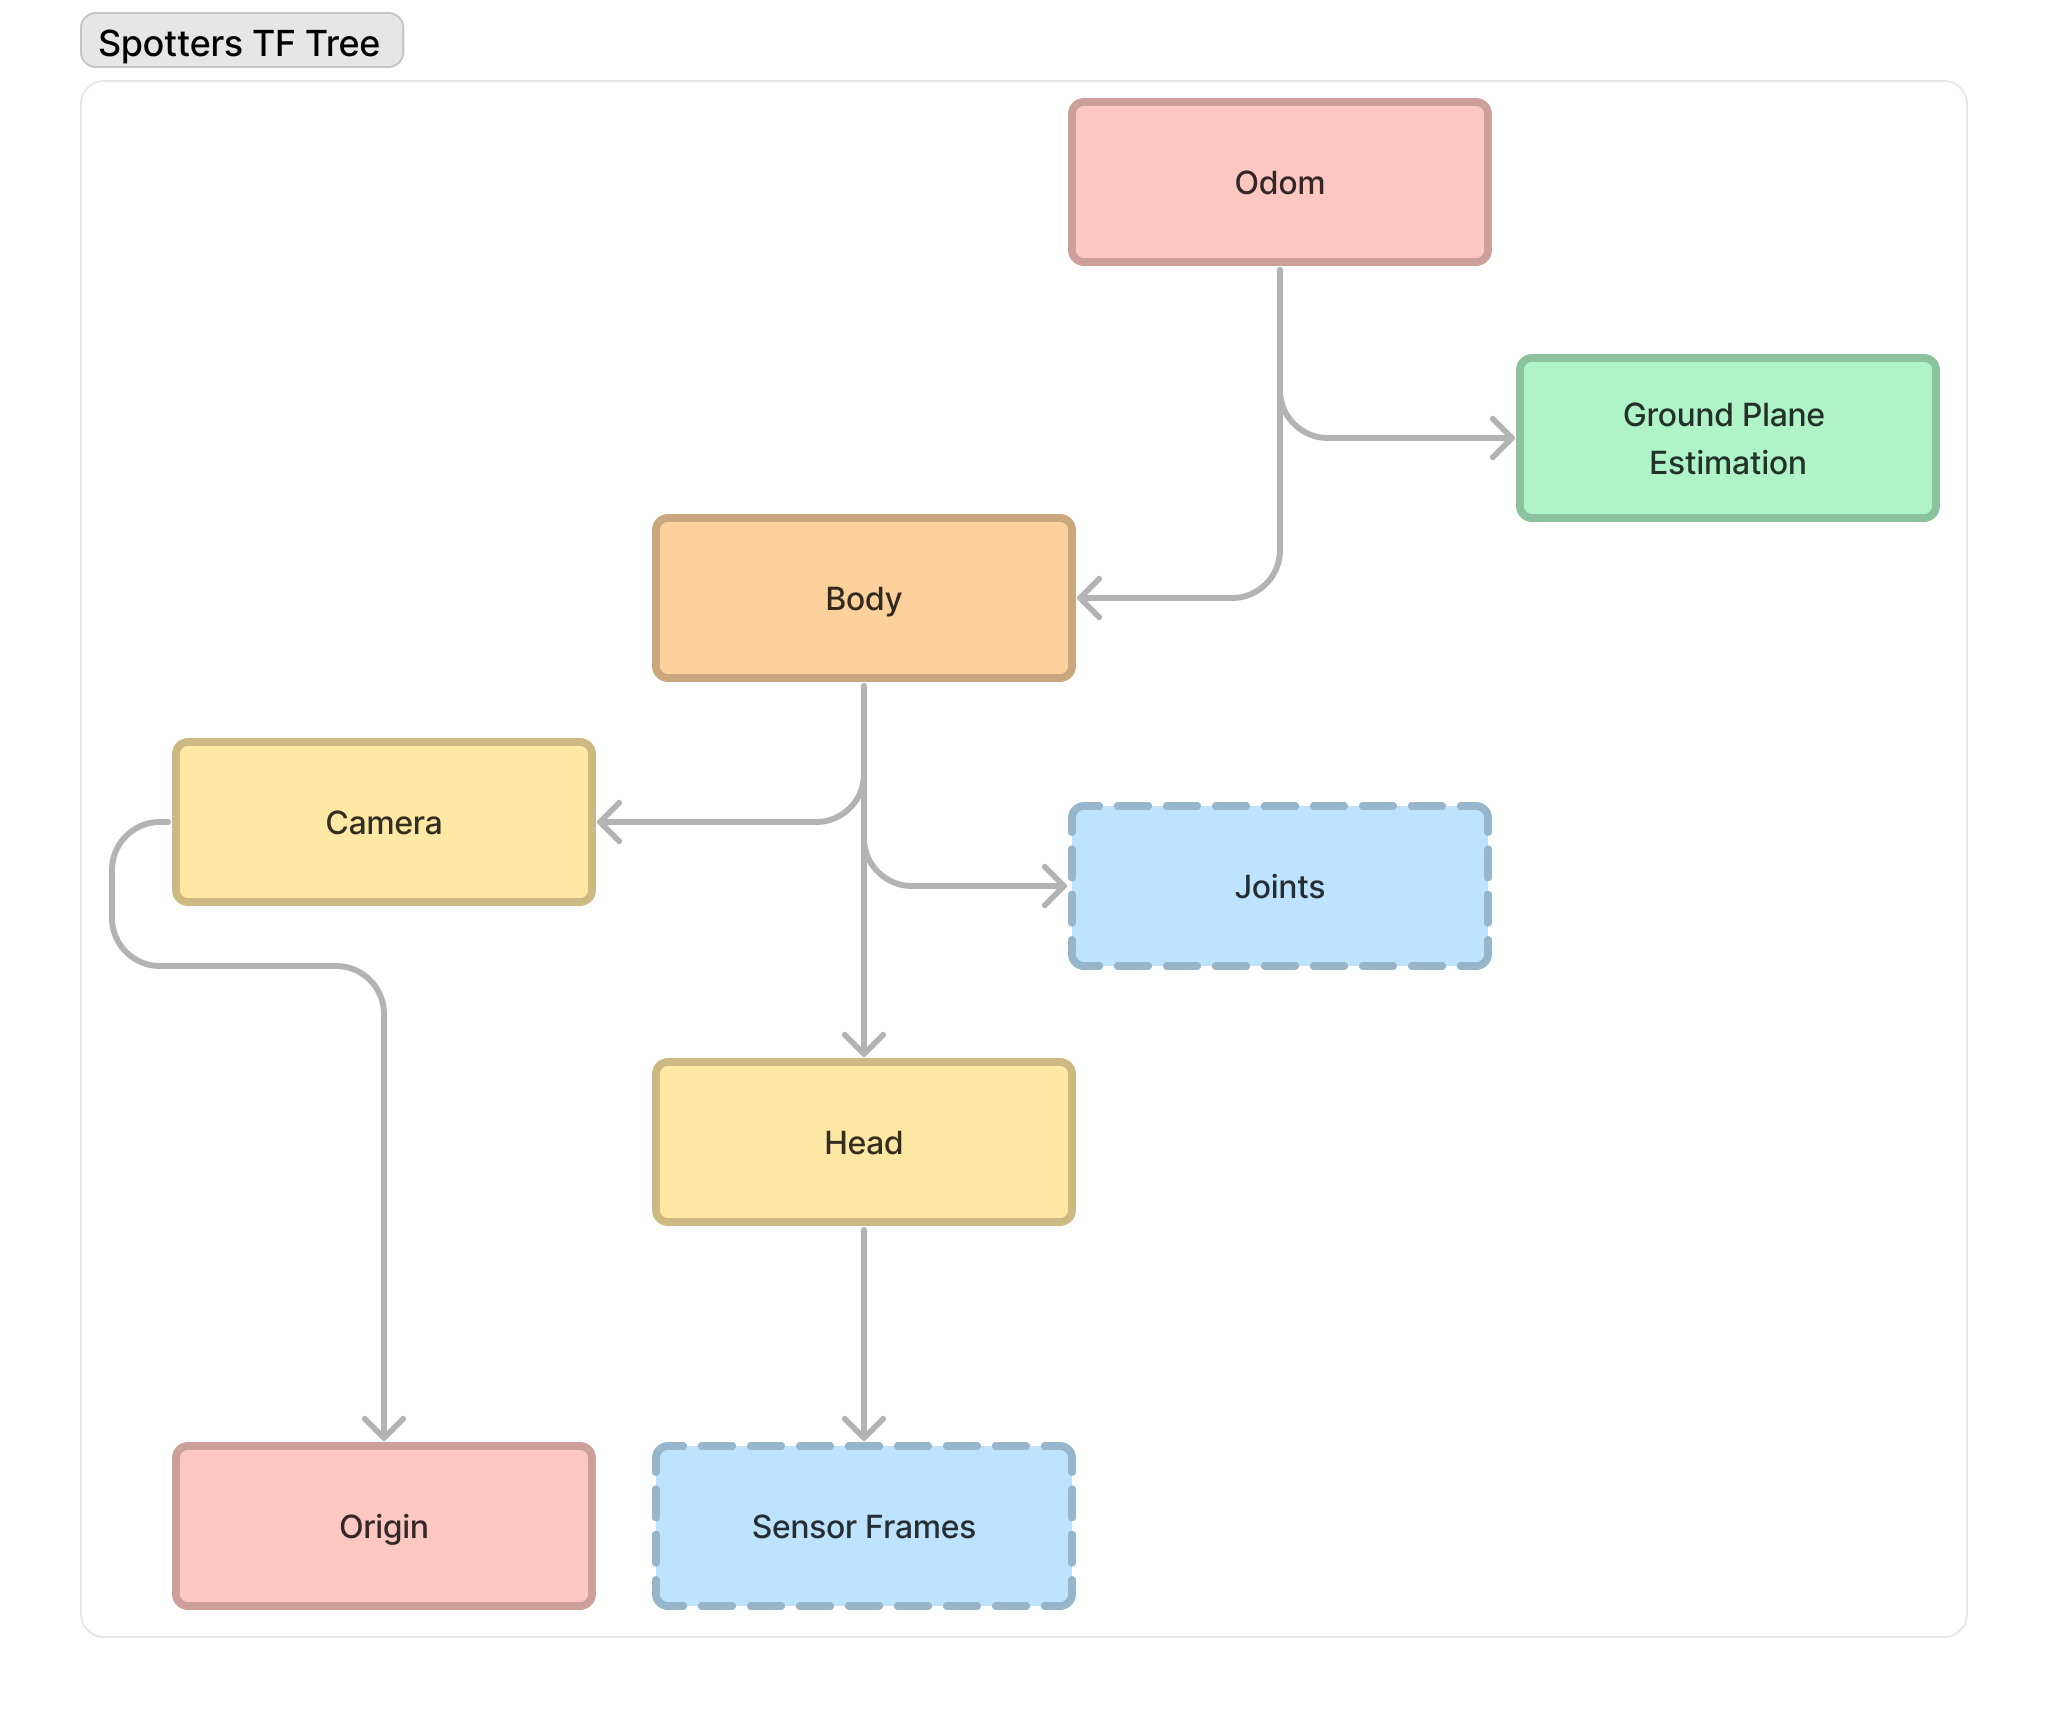
\includegraphics[width=\textwidth]{images/TFTree.png}
    \linebreak
    \text{Diagram of our customised kinematic transform tree.}
\end{center}
\vfill
\thispagestyle{empty}

\subsubsection*{Occupancy Grid Generation}

Our strategy for generating a navigable occupancy grid is a geometric one. First, a two-dimensional slice is taken from the \texttt{octree} point cloud and sent to our mapping pipeline as an \texttt{OccupancyGrid} message. All coordinates where features have been identified are obstructed in the occupancy grid; these coordinates are taken and used as the vertices in our Delaunay triangulation process that producess alpha shapes over sufficiently dense clusters of features. Alpha shapes are collections of linear curves which outline the shape of a finite set of coordinates.

Delaunay triangulation is the production of edges over a set of points such that the edges create triangles and the circumcircles of each triangle do not contain any additional points. The result is effectively a triangular mesh over the two-dimensional slice generated from the point cloud. This mesh is then polygonised -- internal edges are removed and external edges combined into a single shape -- using Python's \texttt{Shapely} library, where each polygon thus represents an intraversible region in the environment. This transforms the sparse point cloud, where walls and other obstructions are often permeable due to the low density of features, into the navigable map where obstructions are contiguous. A configurable alpha value is used to constrain the size of each shape in the triangulation, so points that are sufficiently separated are not subsumed by a single polygon in the next step. At present, this value has been configured manually, but we believe it possible to calculate the optimal alpha for a given set of points. We have not looked into this extensively, though.

Once these occlusion polygons have been generated, we translate the occluded and free space back into a two-dimensional array. Initially, this was done by taking every index and testing if the corresponding coordinate was inside any of the generated polygons using \texttt{within} or \texttt{contains} from the \texttt{Shapely} library. However, this quickly becomes untenable for larger maps because these functions are quite expensive, and confirming that a cell is not occupied requires verifying that it is not inside any polygon. To speed this process up, we have used a data structure from Python's \texttt{rtree} library that performs spatial queries very quickly. By storing all polygons inside this \texttt{rtree}, we can very quickly narrow down the number of polygons that need searching for each point by querying possible matches. We then check each possible match for containment of the point using \texttt{Shapely} as before, where the number of invocations has been substantially reduced.

Once this process is complete and all points in the occupancy grid have been marked as free or occupied, the array is reshaped into one dimension and published as a new \texttt{OccupancyGrid} message. This process allows us to map from a sparse point cloud by treating clusters of features as contiguous, and therefore non-navigable shapes. However, we believe a much faster method exists for deriving the occupancy grid from the generated polygons; we have discussed this as part of our analysis.

\subsubsection*{Navigation}

The navigation pipeline is heavily based on the \texttt{D* Lite} heuristic search algorithm.
We have chosen the \texttt{D* Lite} as our path-finding algorithm since it is considered optimal, complete, and computationally efficient as compared to other path-finding algorithms [2].
Compared to \texttt{A*}, \texttt{D* Lite} is considered more efficient in such complex environments as the interiors of the hospital where paths need to be recalculated as the robot traverses and runs into new obstacles it was not aware of prior.

We have utilised an existing algorithm [3] and modified it so that it can be integrated into the rest of our architecture. The following details how our customised path planner works.

Once the current position, the goal position, and the map are known, the path planner package creates a navigation task object to initiate the path-finding using \texttt{D* Lite}.
Since the existing algorithm uses a two-dimensional array, the published one-dimensional map data need to be reshaped, thereby making it necessary to convert published poses into corresponding rows and columns in the two-dimentional array. Via rostopics, the navigation task (navtask) object stores all the data, converted or original, needed to initiate the path-finding.

Once the navigation task is initiated, the robot's initial movement according to the path generated by \texttt{D* Lite} helps dynamically update the path based on the newfound, neighbouring cells in the viewing range. The viewing range itself is dynamic to the map resolution, tuned to make sure that the robot doesn't waste resources trying to plan too far ahead, but still being able to comfortably walk around obstacles close by. The navigation pipeline then continues to publish updated paths until the current position of the robot is close to the goal position by some constant threshold, after which another navigation task will be created and wait for the necessary data to begin another episode of path-finding. The planner will keep receiving map and current position updates while planning, and the newly created paths will reflect those factors.

Because of the nature of the \texttt{ORB-SLAM3} algorithm, it is likely that the robot will lose its localisation from time to time. To accommodate a situation like this, when we receive the information that the robot is lost, we will set the goal relative to its last known location in order to best preserve the goal. We also make sure to bound our goal position within the map, and the ultimate goal is cached so that we can progressively get closer to it. With D* Lite, every time a new map is received, cells within the viewing range of the current position cell are factored in to generate an updated path. This process is repeated until the final goal is reached.


\subsubsection*{Planning \& Behaviour}

Our \texttt{Conductor} manages the state, and thus the appropriate behaviour, of our robot in its environment. It is effectively an automaton with the following states:

\begin{itemize}[noitemsep]
    \item \texttt{START} is the initial state upon startup. At present, given the absence of any initial navigable map, this state encodes behaviours that helps our visual mapping solution generate one, such as turning around slowly and moving to get different perspectives of the same environment. It combines rotation, with translation in both the X and Y axis, for a predetermined amount of cycles. States outside this one are generally only entered after this initial map has been built. If a map is available, this state transitions to \texttt{GOAL} if a navigation goal has been received, or \texttt{IDLE} otherwise. It's worth noting that these initial behaviours would be made redundant by a more reliable and accurate visual mapping system; we have discussed these details in our analysis. If this behaviour does not manage to form a navigable map, it would repeat until it does so.
    \item \texttt{GOAL} is the state entered upon the receiving a navigation goal, and which persists until either that goal is reached, cancelled, or localisation in the current occupancy grid is lost. The behaviour in this state is navigation toward the given goal position: this is achieved by receiving a path -- either to the coordinate itself, or to the nearest known location in the event that a map of the area doesn't exist yet -- as a sequence of poses from \texttt{Navigation} and dispatching the corresponding gRPC calls to Spot via the \texttt{ros\_wrapper} package.
    \item \texttt{LOST} is the state entered when localisation is lost, and is intended to encode behaviours that will help re-establish localisation, such as looking and moving around to identify features. These behaviours were deemed surplus to requirements for submission, but the framework for their implementation remains. An example of behaviour in this state, would be random movement to nearby unoccupied tiles, until a path is available to the goal.
    \item \texttt{IDLE} is the default state when there is no goal, but there is a healthy map. Currently, there is a chance of SPOT rotating, to emulate life, but otherwise this state is simply waiting.
    \item \texttt{RECOVER} Due to the nature of our SLAM algorithm, there is a reasonable chance that upon map creation, SPOT's position can be on an occupied tile. This is likely due to a lack of data prohibiting the calculation of the ground plane. For this state, rotations can aid in the merging of the map, or collection of new data to 'free' spot from this state.
\end{itemize}

\vspace*{\fill}
\begin{center} % TODO: Finish this state diagram.
    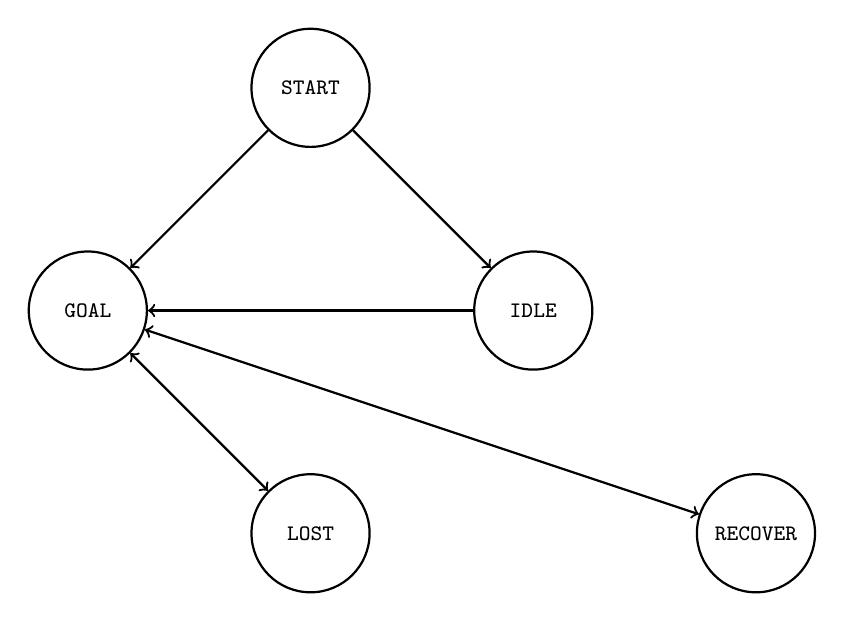
\begin{tikzpicture}[main/.style = {draw, circle}, node distance={40mm}, thick, minimum size=1.5cm]
        \node[main] (1) {\footnotesize \texttt{START}};
        \node[main, below right of=1] (2) {\footnotesize \texttt{IDLE}};
        \node[main, below left of=1] (3) {\footnotesize \texttt{GOAL}};
        \node[main] (4) [below right of=3] {\footnotesize \texttt{LOST}};
        \node[main] (5) [below right of=2] {\footnotesize \texttt{RECOVER}};
        \draw[->] (1) -- (2);
        \draw[->] (1) -- (3);
        \draw[->] (2) -- (3);
        \draw[<->] (3) -- (4);
        \draw[<->] (3) -- (5);
    \end{tikzpicture}
    \linebreak
    \linebreak
    \text{\texttt{Conductor} transition diagram.}
    \text{Not all implemented at the moment, but these are the intended behaviours.}
\end{center}

\clearpage

\section*{Retrospective}

\subsection*{Analysis}

% Analysis of the strengths and weaknesses of the software.
%   Requires:
%   - Excellent analysis of the final deliverable.
%   - Provides a clear understanding of the strengths and weakness of the software.

\subsubsection*{Mapping \& Localisation}

Reliable distance data would, in theory, completely fix the scaling and proportion problems we have encountered due to the estimated distance of features from the monocular camera. With an accurate distance for each of these features, the occupancy grid could be made substantially more realistic and the data from Spot's depth cameras could also be incorporated into a single point cloud. At the moment, this cannot be done because the distances of features in the depth and orb clouds are effectively disjoint, and their fusion would yield a corrupt environment. We have indirect experimental evidence of this conjecture via rosbag testing, where we found that a monocular camera with associated Internal Measurement Unit data produced a much more dispersed point cloud than the quite condensed one produced using just the monocular camera. % TODO: Why?

With more computing power, our initial attempts at mapping may have been more performant. We experimented with the utilization of convex-hulls, and their intersections with alpha-shape geometries informed by the point-clouds to create a 3d naviagation mesh. We believe that our plan was sound, but due to performance constraints we persued a simpler mapping technique. The main advantage to this technique was that it accounts for featureless walls. This turned out to be a non-issue in the Health lab where we demonstrated our project, however it may be a more general solution to our problem.

Another solution to map scaling, as well as a feature mentioned by stake-holders, is the ability to load in an accuratefloor-plan of a building to inform the SLAM algorithm. Converting a floor plan into a dense point cloud, and pre-loading this upon start-up could improve the SLAM algorithm's tracking of walls, and force it to scale features to their real dimensions. This is a logical extension of our current work, and may reduce the necessity for further sensor fusion.

Another area of the mapping pipeline that could have been improved was the usage of an inverted node in the TF tree. While wedid not find or thoroughly expriment with this part of the project, we suspect that there are more conventional ways of achieving what we require: multiple TF trees with a shared body working simultaneously. We require two 'truths' formapping, to isolateSPOT's internalodometr

\subsubsection*{Occupancy Grid Generation}

Whilst our technique for generating a navigable occupancy grid over a sparse point cloud has been serviceable for testing so far, our testing environments have been quite small and open for the most part. We are quite sure that performance would degrade significantly when navigating around a larger map, because more polgons are generated and more points need to be tested for membership of those polygons. So, our current solution does support the deliverable of producing a map of the environment that can be used for navigation, but it is unlikely to scale very well.

The key strength of our technique in this area is the coagulation of clustered points into contiguous polygons that are impermeable from a path planning perspective. This transforms the sparse point cloud generated by our VSLAM algorithm into a useful model of the environment. However, not only are the constituent computations rather expensive, but the entire map is recomputed whenever more data is incorporated from the camera. This means, as mentioned before, that performance degrades sharply for maps of larger areas. Ideally, only a surrounding region of our map would be recomputed for every new frame of information, instead of the whole map, but we have not considered this in depth at this stage.

At the moment, every position in the two-dimensional occupancy grid needs to be checked occlusion by a polygon. As a temporary solution, we have reduced the number of cells checked artificially, by checking every third location across both axes and occluding the nine surrounding cells if an obstruction is found for each check. This is very undesirable in the long term because it drastically reduces map resolution, and could lead to occlusions being undetected or overestimated. This is especially true in the case of doorways, for example, which could become completely blocked in the occupancy grid as a result of this low-resolution sampling. More detail in our occupany grid is also desirable for more accurate modelling and planning in general.

There is also a technique we've theorised for substantially increasing the speed of occupancy grid generation once the polygons have been derived. Python's \texttt{Shapely} library allows for the decomposition of \texttt{Polygon} objects into their boundaries, representated as a collection of lines with start and end coordinates, and for the derivation of points along those lines. If we take all constituent lines in the collection of polygons we generate and derive their coordinates at all integer positions along the line, we can replicate the shape's boundaries in the two-dimensional array by occluding each of these coordinates. Some care would be required to make sure these drawn lines were always connected, but the result would be a functionally continuous outline of all polygons as obstructed positions in the occupancy grid. We can then sample spaces as we do now to see if they are obstructed or unobstructed, and flood fill the surrounding space with the appropriate value. We sampling would continue as long as unknown positions remained in the occupancy grid. We believe this to be a much more efficient approach that, especially when paired with the revision of map subsections instead of total regeneration, would better support the modelling of larger environments and our navigation through them.

\subsubsection*{Navigation}

There are several strengths and weaknesses of the approach with \texttt{D* Lite} implementation.

When provided with a goal that is out of bounds of the currently known area, the navigation system will successfully continue to publish a path plan towards the closest possible point towards the goal until it receives new knowledge about the map, in which case it will re-plan even further towards the goal, allowing for any kind of dynamic maps. Another strong point is that it successfully handles all situations where the robot might be out of bounds, or no path could be planned, and alerts the user during such conditions by publishing its status to a topic. In those cases, no new path will be published, as trying to do so might result in the robot not reaching the goal correctly. This leads to the navigation system being able to tolerate and handle situations where the map being published is not completely accurate. Finally, the last notable point is the dynamic goal system. When the map is lost and a new one is generated after, the navigation system will recognize this and adjust the old goal position to a relative distance, which is the distance between the last known position and the goal. This allows the goal to persist even when the map is lost, and in some cases, even recover from being lost by following the path generated from the relative distance.

However, there are also weaknesses with the current approach, of which one would be sync problems with the other publishers relating to the map being lost. When the robot gets lost, the old map would be temporarily set aside until the robot successfully localizes and merges the maps back together. This is an issue, as when a path calculation happens at the same time as the map is being replaced with a completely new one, the planner might be really off, or simply not work at all due to it reading the modified data halfway through the calculation. This issue is an edge case and will not happen often. A theorised way to fix this would be to turn off everything related to updating the map while the path calculation is being done. While this will fix the planner stopping, it might generate a wrong path if the robot is lost by a huge displacement until the next time path is calculated, and as such, is not a perfect solution.

\clearpage

\subsection*{Evaluation}

% Critical evaluation of the project in relation to the negotiated requirements.
% Quality of quantitative and/or qualitative experimental results.
%   Requires:
%   - Excellent evaluation of the capabilities of the final deliverable.
%   - Well-supported experimental evidence.

\subsubsection*{Mapping and Localisation}

We made several compromizes to improve the performance of our mapping pipeline. Primarily, we were reducing a three dimensional octree, into a two-dimensional slice for the creation of the OccupancyGrid. Keeping the octree three-dimension, and changing the navigation stack to accomodate this would have allowed our solution to have the data required to perform tasks such as climbing stairs, or moving underneath obstacles. As we were already storing the data in three dimensions, this change would not significantly effect performance.

To accomodate this, navigation would have to be extended with logic to determine what the navigable area is. An example of this logic would be to first determine which octree tiles the robot is standing on top of, then flood-filling outwards to all other walkable tiles. Some knowledge of the heights that SPOT can climb, and the obstacles that spot can duck under would improve the fidelity of this flood fill\dots

Additionally, For the demonstration we had almost implemented sensor fusion, utilizing a monocular camera, IMU data from the attached phone, and SPOT's depth cloud data. This would have significantly increased the accuracy of the resultant map, particularly for scale, wall detection and localization. The IMU data is required to match the scale of the monocular camera, which would then make combining the SLAM point-clouds with the depth data appropriate. This depth data is a 'dense' point cloud, meaning that we do not have to employ novel techniques to accomodate featureless walls.

\subsubsection*{Occupancy Grid Generation}

Overall, the technique we've used for generating a navigable occupancy grid over a sparse point cloud has been sufficient for the robot to map and navigate its environment as per the negotiated requirements. Whilst navigation's implementation and integration with the rest of the system isn't particularly robust at present, the map we generate is capable of supporting the derivation of realistic paths through a given environment, which is its primary function. The scale of the environment are very inaccurate due to the limitations of our monocular camera, however the general shape is represented correctly in most cases. Integration of reliable depth data from the camera is the primary means by which this deliverable could be improved upon, because the more accurate map available to us using depth data would support more robust exploration.

Our initial exploration into the problem started with the development of 3d meshes for navigation. We diverted from this approach early, as we predicted that we would run into time and hardware blockers. Despite this, the 3rd dimension remains important for SPOT's navigation. As our input point-clouds are inherently three dimensional, converting these into a 3d mesh, or simply using a 3d octree as a navmesh are an obvious extension to our current implementation. We did not implement this due to added complexity for navigation, but we believe this would be a valuable extension to the current codebase.

\vspace*{\fill}
\begin{center}
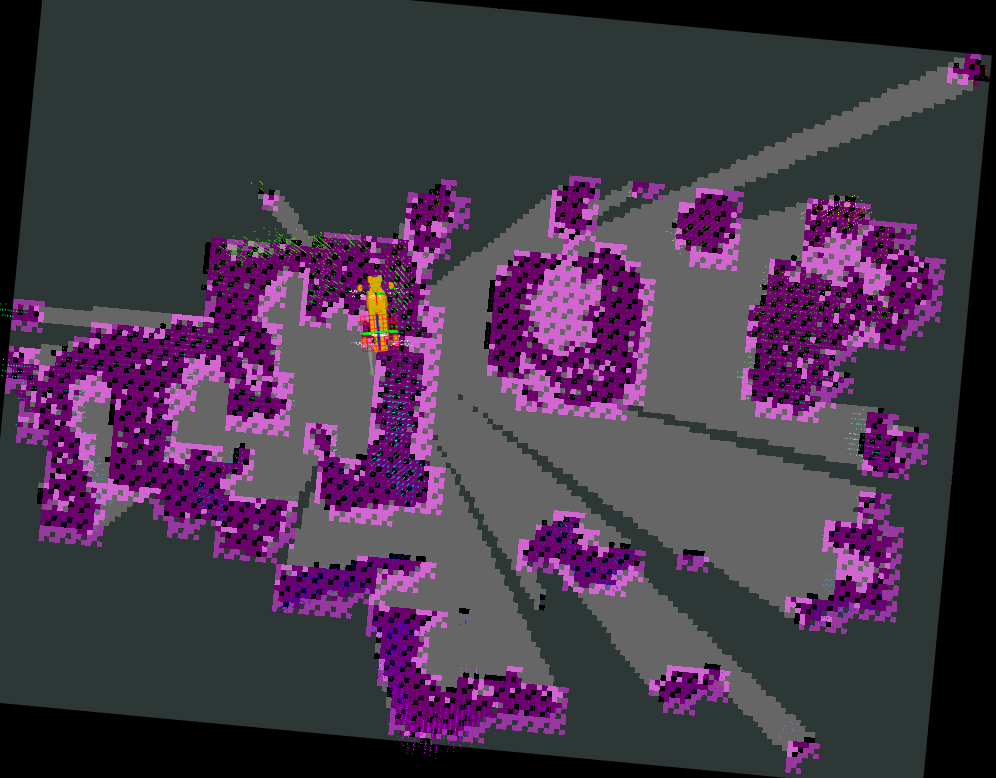
\includegraphics[width=0.6\textwidth]{images/BigMap.png}
\linebreak
\linebreak
\text{A larger map, such as this one, is not efficiently computable in real time.}
\text{This required almost a minute to generate from each frame as the map approached this size.}
\end{center}
\vfill

\subsubsection*{Navigation}

The navigation part within the project pipeline has done an adequate job of providing the robot with the path it needs to take towards the goal. Tests were run using a tool called \textit{rosbag}, which allows ROS topics to be recorded and replayed at anytime. Within these testing environments, various conditions were tested to see whether the navigation system would come up with the correct paths:

\begin{enumerate}[noitemsep]
    \item Attempting to plan a path when there is a clear path available. This results in a path being generated as expected, generating a path around obstacles within viewing range, but not looking too far ahead. % NEED PICTURES REFERENCED
    \item Attempting to plan a path out of bounds. This results in a path being generated to the edge of the known area leading towards the goal, which is the expected behaviour.
    \item Attempting to plan into an obstacle outside of viewing range. This results in a path being generated as if there were no obstacles. When the goal comes into viewing range, the navigation system decides that no path is possible and stops planning, which is the ideal behaviour.
    \item Attempting to plan a path towards a goal, then getting lost. After receiving the new dummy map, the system sets the goal to a distance relative to where it was before getting lost, which is the intended behaviour of the goal persistence behaviour.
\end{enumerate}

Later on, tests would be run directly on the robot itself while following the path with similar outcomes. An issue that pops up is that the robot would get lost often and the navigation system would become imprecise. Further extensions to the navigation algorithm include the integration of a string-pull algorithm, which would result in fewer, more significant legs of each path. This would solve some issues we experienced with short, abrupt sections of movement, which would be replaced by long, direct length of travel. Additionally, the development of a front-end to simply end-user interaction with the navigation goals would be beneficial for the utilization of SPOT in the health lab.

\vspace*{\fill}
\begin{center}
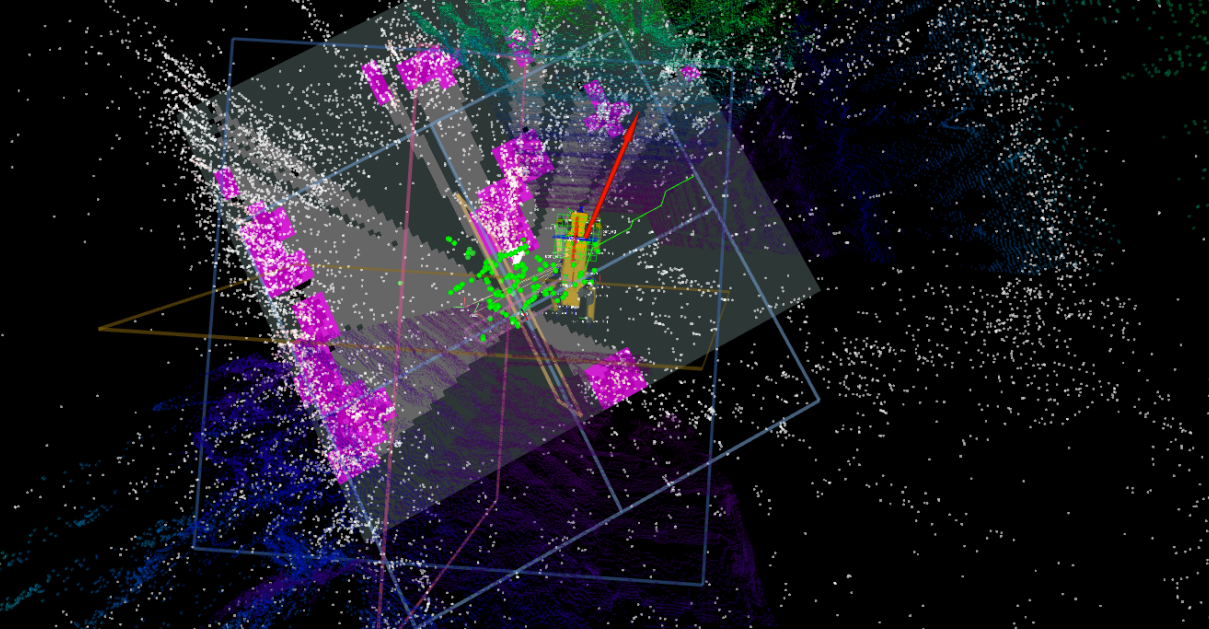
\includegraphics[width=0.5\textwidth]{images/Path1.png}
\linebreak
\linebreak
\text{Green \texttt{D* Lite} path does not extend beyond the known map.}
\end{center}
\vfill
\thispagestyle{empty}

\clearpage

\vspace*{\fill}
\begin{center}
\includegraphics[scale=0.1]{images/429F1310-292D-47FB-AB48-3564D69C3279.png}
\linebreak
\linebreak
\text{Attempting to calibrate the IMU data in Raf's iPhone.}
\end{center}
\vfill
\thispagestyle{empty}
\clearpage

\section*{Literature}

\subsubsection*{Structure PLP-SLAM: Efficient Sparse Mapping and Localization using Point, Line and Plane for Monocular, RGB-D and Stereo Cameras}

This paper details a novel method to tackle a similar problem that we faced with our sparse point cloud data. While OrbSLAM tracks feature points, Stucture PLP-SLAM detects edges and faces in RGB camera data, and determines the orientation of these faces.

By matching straight lines (edges) to faces, PLP-SLAM can map entire walls that would otherwise be featureless for OrbSLAM. This tracking of whole faces is advantageous for navigation in sterile environments, however we suspect that it's benefits are less so in more visually complex environments, suited to feature detection. The classification of edges and faces seems highly advantageous for any SLAM algorithm, and we would aim to implement a similar approach for an indoor-specific platform, such as SPOT for a hospital.

\subsubsection*{Building maps for autonomous navigation using sparse visual SLAM features}

This paper focuses on SLAM-exclusive map building for car based navigation. It builds a 3d polygonal navigation method by 'carving' from the camera, out to known features. This results in a decent quality,'water-tight' mesh suitable for navigation. This implementation is closer to what our initial attempt was going to be, which we determined was too resource intensive. After reviewing this paper, we can determine that there are more computationally efficent methods for creating 3d nav-meshes. We believe that this approach would be suited for indoor mapping, in addition to the road maps depicted in the paper. However we are not sure about the 'first-time' performance of this algorithm,or how it would handle the exploration of a new space.We do see some unnavigable artifacts on areas that would otherwise be empty ground. These would be navigable with out solution. We suspect that these issues would be resolved over time by their polygonal mapping algorithm.

\clearpage

\section*{Contributions}  % Add your contributions here.

\subsection*{Raf}

Rafat's contributions include initial phone-based prototyping of the OrbSlam algorithm, architectural designs for the whole system, integration of the \texttt{spot\_ros} API, movement pipeline, IMU integration and testing on the SPOT robot.

\subsection*{Adrian}

Adrian's main contributions were in the Mapping and Conductor pipelines, data alignment for integrating the mapping solution, as well as contributing to the initial architecture and system diagrams. Significant time was spent integrating code into the physical robot, and testing our solutions of the end hardware.

\subsection*{Harry}

Harry's main contributions were in initial experimentation tinto SLAM implementations, mapping solutions and imu integration. In addition, Harry contributed to refactoring the mapping, and conductor pipelines, and aided in integration for the SPOT robot.

\subsection*{David}

David's main contributions were in the Navigation pipeline, as well as contributing to the initial setup of running programs on the robot. A lot of the time went into integrating the navigation into ROS, adding guards in order to prevent crashes in unfavourable situations, and the transformations of the coordinates.

\subsection*{Myeonghoon}

Myeonghoon's main contributions were the development of the navigation pipeline, establishing standards for topic processing between nodes, and integration of the D*Lite algorithm.

\clearpage

\section*{References}

\begin{enumerate}[leftmargin=*,label={\texttt{[\arabic*]}},noitemsep]
    \item C. Campos, R. Elvira, J. J. G. Rodríguez, J. M. M. Montiel and J. D. Tardós, ``ORB-SLAM3: An Accurate Open-Source Library for Visual, Visual-Inertial, and Multimap SLAM,'' in IEEE Transactions on Robotics, vol. 37, no. 6, pp. 1874-1890, Dec. 2021, doi:\\10.1109/TRO.2021.3075644.
    \item P. E. Teleweck and B. Chandrasekaran, ``Path planning algorithms and their use in robotic navigation systems,'' Journal of Physics: Conference Series, vol. 1207, p. 012018, 2019, doi:10.1088/1742-6596/1207/1/012018
    \item Sollimann, ``Sollimann/Dstar-Lite-pathplanner: Implementation of the D* lite algorithm in python for `Improved fast replanning for robot navigation in unknown terrain,''' GitHub, https://github.com/Sollimann/Dstar-lite-pathplanner (accessed Jun. 16, 2023).
    \item Y. Ling and S. Shen, ``Building maps for autonomous navigation using sparse visual SLAM features,'' \textit{2017 IEEE/RSJ International Conference on Intelligent Robots and Systems (IROS),} Vancouver, BC, Canada, 2017, pp. 1374-1381.
    \item F. Shu, J. Wang, A. Pagani, D. Stricker,  ``Structure PLP-SLAM: Efficient Sparse Mapping and Localization using Point, Line and Plane for Monocular, RGB-D and Stereo Cameras'' 2022
    https://arxiv.org/abs/2207.06058 (Accessed: 25 May 2023).
\end{enumerate}

\end{document}
